\section{Bewertung der Daten in Grafana}

%Mit dieser Arbeit wollten wir eine \gls{opensource} ähnliche \gls{SIEM} Lösung verwenden, um Überwachungsmechanismen über Logdateien zu erstellen. Die folgende Tabelle vergleicht die existierenden Funktionalitäten eines \gls{SIEM} mit denen, die wir mit unserem Aufbau erreichten:

In dieser Arbeit haben wir versucht, eine \gls{opensource}-basierte Lösung ähnlich einem \gls{SIEM} zu verwenden, um Überwachungsmechanismen anhand von Logdateien zu erstellen. In der folgenden Tabelle vergleichen wir die vorhandenen Funktionalitäten eines \gls{SIEM} mit denen, die wir durch unsere Implementierung erreichen konnten.

\begin{table}[H]
    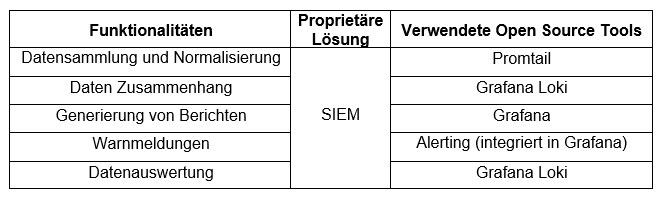
\includegraphics[width=\linewidth]{assets/tabelle_siem_BA.png}
    \caption{Verwendete Tools für den Aufbau einer \gls{SIEM} ähnlichen Lösung\\Quelle: Eigene Quelle und \citep{Granadillo_SIEM}}
 \end{table}
 
%Aus einer prinzipiellen Sicht können wir behaupten, dass die verwendeten Tools eine kostengünstige Möglichkeit anbieten, eine Überwachungssystem in einem Rechenzentrum zu implementieren. Die Methoden für Angriffserkennung lassen sich von der \gls{mitre} Matrix oder von anderen Framework deutlich definieren. Nach der Auswhal des Angriffes, erstellen wir Regelsätze mit der Abfragesprache \gls{logql} in Loki, um Muster zu identifieren, die auf den ausgewählten Angriff hindeuten. Wir benutzen dann diese Regelsätze, um Warnmeldung über den Angriff zu generieren und zu schicken.

Aus prinzipieller Sicht können wir feststellen, dass die verwendeten Tools eine kosteneffektive Möglichkeit bieten, ein Überwachungssystem in einem Rechenzentrum zu implementieren. Die Methoden zur Erkennung von Angriffen lassen sich klar anhand der \gls{mitre}-Matrix oder anderer Frameworks definieren. Nach der Auswahl des Angriffs erstellen wir Regelwerke mit der Abfragesprache \gls{logql} in Loki, um Muster zu identifizieren, die auf den ausgewählten Angriff hindeuten. Diese Regelwerke werden dann verwendet, um Warnmeldungen über den Angriff zu generieren und zu versenden.

%Unser Aufbau hat zwei große Herausforderungen. Die erste lässt sich einfacher beseitigen als die zweite. Diese sind:

Unser Aufbau birgt zwei große Herausforderungen, wobei die erste einfacher zu bewältigen ist als die zweite. Diese sind:

\begin{itemize}[noitemsep]
    \item \textbf{Definition der Regelsätzen}
\end{itemize}

%Für eine präzise Implementierung spielt die richtige Entwicklung der Regelsätzen für die Identifizierung des potenziellen Angriffes eine wesentliche Rolle. Da Logdateien aus produktiven Umgebungen große Menge von Information beinhalten, müssen diese Regelsätze so festgelegt werden, dass sie die eindeutige Informationen, wie IP-Adresse, Portnummer, Zeitfenster und Abstandzeit zwischen Anfrage, filtern und nach Angriffsmuster kategorisieren.

Für eine präzise Implementierung spielt die richtige Entwicklung der Regelsätzen zur Identifizierung potenzieller Angriffe eine wesentliche Rolle. Da Logdateien aus produktiven Umgebungen eine große Menge an Informationen enthalten, müssen diese Regelsätzen so definiert werden, dass sie die eindeutigen Informationen wie IP-Adresse, Portnummer, Zeitfenster und Zeitabstände zwischen Anfragen filtern und nach Angriffsmustern kategorisieren können.

\begin{itemize}[noitemsep]
    \item \textbf{statische Regel in einer dynamischen Angriffswelt}
\end{itemize}

Die von uns definierten Regel haben statische Elementen, wie \quotes{Anzahl von Anfrage}, \quotes{Zeitabstand zwischen Requests}, \quotes{Anzahl von fehlgeschlagenen Anmeldeversuchen}. Die heutigen Angriffe haben aber einen dynamischen Aspekt, die sich an der Umgebung anpasst. \gls{polyphomicMalware} nur ein Beispiel blabla bla
sind nur eins von vielen Beispiele, die nicht 

\begin{itemize}[noitemsep]
    \item Zielen
    \item Ergenissen
    \item Herausforderungen
 \end{itemize}
 
\subsection{Zukünftige Entwicklungen}

\begin{itemize}[noitemsep]
    \item Dynamische Regel
    \item Maschine Learning
    \item Grafana Nutzung einschränken
 \end{itemize}
 
